\documentclass[12pt,a4paper]{article}

% ── Core packages ──────────────────────────────────────────────────────────────
\usepackage{amsmath, amssymb}
\usepackage[margin=2.5cm]{geometry}
\usepackage{booktabs}
\usepackage{xcolor}
\usepackage{hyperref}
\usepackage{listings}
\usepackage{pgfplots}
\pgfplotsset{compat=1.18}
\usepackage[most,breakable]{tcolorbox}
\tcbuselibrary{skins, breakable}
\usepackage{enumitem}
\usepackage{fancyhdr}
\usepackage{tikz}
\usepackage{array}

% ── tcolorbox environments ─────────────────────────────────────────────────────
\newtcolorbox{curiositybox}[1]{colback=yellow!10, colframe=orange!80!black,
  fonttitle=\bfseries, title=#1, breakable}
\newtcolorbox{infobox}[1]{colback=blue!5, colframe=blue!60!black,
  fonttitle=\bfseries, title=#1, breakable}
\newtcolorbox{mistakebox}[1]{colback=red!5, colframe=red!60!black,
  fonttitle=\bfseries, title=#1, breakable}
\newtcolorbox{learnbox}[1]{colback=green!5, colframe=green!60!black,
  fonttitle=\bfseries, title=#1, breakable}

% ── lstlisting configuration ───────────────────────────────────────────────────
\lstset{language=Python, basicstyle=\ttfamily\small, keywordstyle=\color{blue},
        commentstyle=\color{gray}, stringstyle=\color{orange},
        showstringspaces=false, numbers=left, numberstyle=\tiny,
        breaklines=true, frame=single}

% ── fancyhdr ───────────────────────────────────────────────────────────────────
\pagestyle{fancy}
\fancyhf{}
\lhead{Topic 08: Periodic Function Transforms}
\rhead{Unit IV --- Laplace Transforms}
\cfoot{\thepage}

% ── Title metadata ─────────────────────────────────────────────────────────────
\title{Topic 08: Laplace Transform of Periodic Functions \\
  \large Unit IV --- Laplace Transforms}
\author{23A54201 --- Mathematics IV (Transform Techniques) \\
  JNTUA College of Engineering (Autonomous)}
\date{}

% ══════════════════════════════════════════════════════════════════════════════
\begin{document}
\maketitle
\tableofcontents
\newpage

% ─────────────────────────────────────────────────────────────────────────────
\section{Opening Hook}
% ─────────────────────────────────────────────────────────────────────────────
\begin{curiositybox}{Hook}
A power supply circuit outputs a square wave that switches between 0V and 5V
every millisecond, forever. Integrating $e^{-st}$ times this wave from 0 to
infinity sounds like an infinite nightmare of piecewise integration --- unless
you notice something beautiful: the wave repeats EXACTLY every period. That
repetition means we only ever need to integrate over ONE period, then let a
simple geometric series formula handle the rest of eternity for us.
\end{curiositybox}

% ─────────────────────────────────────────────────────────────────────────────
\section{Why This Topic Exists}
% ─────────────────────────────────────────────────────────────────────────────

Before we begin, here is the honest answer to why you are reading this.
Periodic signals --- square waves, sawtooth waves, rectified sine waves ---
appear constantly in electrical and mechanical engineering: power inverters,
function generators, vibrating machinery, audio synthesisers. Computing their
Laplace transform directly by writing out an infinite piecewise integral and
summing every piece by hand is \emph{possible} but thoroughly impractical.
The periodic function theorem gives us a clean closed-form shortcut: integrate
over \emph{one} period, divide by $(1 - e^{-sT})$, and you are done.

Here is what goes wrong when students skip this formula:

\begin{center}
\begin{tabular}{@{}ll@{}}
\toprule
\textbf{Mistake / Shortcut attempted} & \textbf{Consequence} \\
\midrule
Attempting direct infinite-interval integration & Getting stuck in an infinite sum without a closed form \\
Forgetting the $(1-e^{-sT})$ denominator & Getting only the first-period contribution, missing all repeats \\
Using wrong period $T$ from the graph & Completely wrong formula substitution \\
\bottomrule
\end{tabular}
\end{center}

\begin{learnbox}{Why This Section Matters}
Three common errors each lead to a completely wrong answer. The theorem exists
precisely to bypass the infinite-sum trap. Knowing \emph{why} it is needed
makes it far easier to remember.
\end{learnbox}

% ─────────────────────────────────────────────────────────────────────────────
\section{You Already Know This (Intuition First)}
% ─────────────────────────────────────────────────────────────────────────────

Imagine you have taken a home loan and every month you pay an EMI (equated
monthly instalment) of Rs.\ 10{,}000. Because money received later is worth
less (due to interest), economists ``discount'' each future instalment by a
factor $r < 1$ per month. The \emph{total present value} of all future
instalments is:
\[
  10{,}000 + 10{,}000\,r + 10{,}000\,r^2 + \cdots
  = \frac{10{,}000}{1 - r}, \quad |r| < 1.
\]
This is just the geometric series formula. You only need to know the value of
\emph{one} instalment and the discount factor $r$.

Now replace ``one EMI'' with ``the integral of $e^{-st}f(t)$ over one period
$[0,T]$'', and replace the discount factor $r$ with $e^{-sT}$ (the Laplace
attenuation over one period). The total Laplace transform is:
\[
  \mathcal{L}\{f(t)\}
  = \frac{\displaystyle\int_0^T e^{-st} f(t)\,dt}{1 - e^{-sT}}.
\]
That is the entire theorem. The rest of this topic is just making this precise
and practising it.

% ─────────────────────────────────────────────────────────────────────────────
\section{Definition of a Periodic Function}
% ─────────────────────────────────────────────────────────────────────────────

\begin{infobox}{Definition: Periodic Function}
A function $f(t)$ defined for $t \ge 0$ is said to be \textbf{periodic with
period} $T > 0$ if
\[
  f(t + T) = f(t) \quad \text{for all } t \ge 0.
\]
The smallest such positive $T$ is called the \textbf{fundamental period}.
Common examples:
\begin{itemize}[noitemsep]
  \item Square wave (period $T$): alternates between two constant values.
  \item Sawtooth wave (period $T$): rises linearly then drops abruptly.
  \item Triangular wave (period $T$): rises then falls linearly.
  \item Full-wave rectified sine: $|\sin(\omega t)|$, period $\pi/\omega$.
\end{itemize}
\end{infobox}

\subsection*{Graph: Square Wave with Period $T = 2$}

\begin{center}
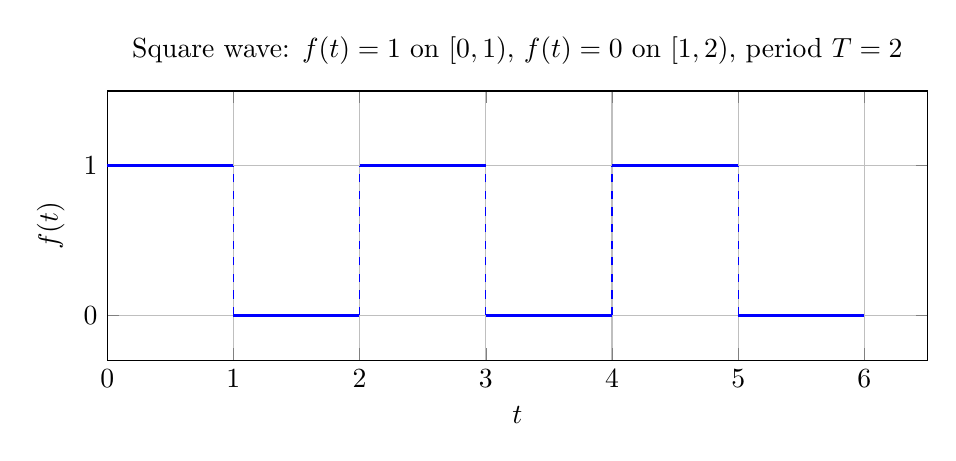
\begin{tikzpicture}
\begin{axis}[
  xlabel={$t$},
  ylabel={$f(t)$},
  xmin=0, xmax=6.5,
  ymin=-0.3, ymax=1.5,
  xtick={0,1,2,3,4,5,6},
  ytick={0,1},
  grid=major,
  width=12cm, height=5cm,
  title={Square wave: $f(t)=1$ on $[0,1)$, $f(t)=0$ on $[1,2)$, period $T=2$}
]
% Period 1: [0,1) -> 1, [1,2) -> 0
\addplot[blue, very thick] coordinates {(0,1)(0.999,1)};
\addplot[blue, very thick] coordinates {(1,0)(1.999,0)};
% Period 2: [2,3) -> 1, [3,4) -> 0
\addplot[blue, very thick] coordinates {(2,1)(2.999,1)};
\addplot[blue, very thick] coordinates {(3,0)(3.999,0)};
% Period 3: [4,5) -> 1, [5,6) -> 0
\addplot[blue, very thick] coordinates {(4,1)(4.999,1)};
\addplot[blue, very thick] coordinates {(5,0)(5.999,0)};
% Vertical transitions (dashed)
\addplot[blue, dashed] coordinates {(1,0)(1,1)};
\addplot[blue, dashed] coordinates {(2,0)(2,1)};
\addplot[blue, dashed] coordinates {(3,0)(3,1)};
\addplot[blue, dashed] coordinates {(4,0)(4,1)};
\addplot[blue, dashed] coordinates {(5,0)(5,1)};
\end{axis}
\end{tikzpicture}
\end{center}

The graph shows 3 full periods of a square wave. Each period is identical ---
this is the key property the theorem exploits.

% ─────────────────────────────────────────────────────────────────────────────
\section{The Periodic Function Theorem}
% ─────────────────────────────────────────────────────────────────────────────

\begin{infobox}{Theorem: Laplace Transform of a Periodic Function}
Let $f(t)$ be a piecewise continuous, periodic function with period $T > 0$
that is of exponential order. Then its Laplace transform exists for $s > 0$
and is given by:
\[
  \boxed{\mathcal{L}\{f(t)\} = \frac{1}{1 - e^{-sT}} \int_0^T e^{-st}\,f(t)\,dt}
\]

\textbf{Key observations:}
\begin{itemize}[noitemsep]
  \item The integral is taken over \emph{only one period} $[0, T]$.
  \item The factor $\dfrac{1}{1-e^{-sT}}$ sums the contributions of all
        infinitely many periods via the geometric series.
  \item For $s > 0$, we have $0 < e^{-sT} < 1$, so the denominator is
        positive and the formula is valid.
\end{itemize}
\end{infobox}

% ─────────────────────────────────────────────────────────────────────────────
\section{Proof of the Theorem}
% ─────────────────────────────────────────────────────────────────────────────

\begin{infobox}{Step-by-Step Proof}
\textbf{Step 1: Split the integral at period boundaries.}

By definition,
\[
  \mathcal{L}\{f(t)\} = \int_0^\infty e^{-st} f(t)\,dt
  = \sum_{n=0}^{\infty} \int_{nT}^{(n+1)T} e^{-st} f(t)\,dt.
\]

\textbf{Step 2: Substitute $\tau = t - nT$ in the $n$-th integral.}

When $t = nT$, $\tau = 0$; when $t = (n+1)T$, $\tau = T$. Also $dt = d\tau$
and $t = \tau + nT$. Therefore:
\[
  \int_{nT}^{(n+1)T} e^{-st} f(t)\,dt
  = \int_0^T e^{-s(\tau+nT)} f(\tau + nT)\,d\tau.
\]

\textbf{Step 3: Use periodicity $f(\tau + nT) = f(\tau)$.}

\[
  = \int_0^T e^{-s\tau} e^{-snT} f(\tau)\,d\tau
  = e^{-snT} \int_0^T e^{-s\tau} f(\tau)\,d\tau.
\]

\textbf{Step 4: Factor out the one-period integral.}

Let $I_1 = \displaystyle\int_0^T e^{-s\tau} f(\tau)\,d\tau$ (constant with
respect to $n$). Then:
\[
  \mathcal{L}\{f(t)\}
  = \sum_{n=0}^{\infty} e^{-snT} \cdot I_1
  = I_1 \sum_{n=0}^{\infty} \bigl(e^{-sT}\bigr)^n.
\]

\textbf{Step 5: Sum the geometric series.}

The series $\displaystyle\sum_{n=0}^{\infty} r^n = \dfrac{1}{1-r}$ converges
for $|r| < 1$. Here $r = e^{-sT}$ and, for $s > 0$, $0 < e^{-sT} < 1$.
Therefore:
\[
  \mathcal{L}\{f(t)\}
  = I_1 \cdot \frac{1}{1 - e^{-sT}}
  = \frac{1}{1 - e^{-sT}} \int_0^T e^{-st} f(t)\,dt. \qquad \square
\]
\end{infobox}

\begin{learnbox}{Proof Summary}
The proof reduces an infinite integral to a finite one via the substitution
$\tau = t - nT$ (which uses periodicity) and then applies the geometric series
formula. Every step is elementary once you make that substitution.
\end{learnbox}

% ─────────────────────────────────────────────────────────────────────────────
\section{Worked Examples}
% ─────────────────────────────────────────────────────────────────────────────

% ── Example 1 ──────────────────────────────────────────────────────────────
\begin{infobox}{Example 1: Laplace Transform of a Square Wave}
\textbf{Problem.} Find $\mathcal{L}\{f(t)\}$ for the square wave defined by
\[
  f(t) = \begin{cases} 1, & 0 \le t < 1, \\ 0, & 1 \le t < 2, \end{cases}
  \quad f(t+2) = f(t).
\]

\textbf{Period:} $T = 2$.

\textbf{Step 1: Set up the one-period integral.}
\[
  I_1 = \int_0^2 e^{-st} f(t)\,dt
  = \int_0^1 e^{-st} \cdot 1\,dt + \int_1^2 e^{-st} \cdot 0\,dt
  = \int_0^1 e^{-st}\,dt.
\]

\textbf{Step 2: Evaluate the integral.}
\[
  I_1 = \left[\frac{e^{-st}}{-s}\right]_0^1
  = \frac{e^{-s \cdot 0}}{s} - \frac{e^{-s \cdot 1}}{s}
  = \frac{1 - e^{-s}}{s}.
\]

\textbf{Step 3: Apply the periodic function theorem.}
\[
  \mathcal{L}\{f(t)\}
  = \frac{I_1}{1 - e^{-sT}}
  = \frac{\dfrac{1-e^{-s}}{s}}{1 - e^{-2s}}.
\]

\textbf{Step 4: Simplify using the difference of squares.}

Note $1 - e^{-2s} = (1 - e^{-s})(1 + e^{-s})$. So:
\[
  \mathcal{L}\{f(t)\}
  = \frac{1 - e^{-s}}{s(1 - e^{-s})(1 + e^{-s})}
  = \frac{1}{s(1 + e^{-s})}.
\]

\textbf{Final answer:}
\[
  \mathcal{L}\{f(t)\} = \frac{1}{s(1 + e^{-s})}.
\]
\end{infobox}

\begin{learnbox}{What Did We Learn? (Example 1)}
For a square wave of amplitude 1 and period 2 (on for half the period), the
transform simplifies neatly to $\dfrac{1}{s(1+e^{-s})}$ after factoring the
denominator. Always check whether $(1-e^{-nT})$ factors with the numerator.
\end{learnbox}

% ── Example 2 ──────────────────────────────────────────────────────────────
\begin{infobox}{Example 2: Laplace Transform of a Sawtooth Wave}
\textbf{Problem.} Find $\mathcal{L}\{f(t)\}$ for the sawtooth wave
$f(t) = t$ on $[0, T)$, repeating with period $T$.

\textbf{Step 1: One-period integral.}
\[
  I_1 = \int_0^T e^{-st} \cdot t\,dt.
\]

\textbf{Step 2: Integrate by parts} (let $u = t$, $dv = e^{-st}\,dt$).
\[
  I_1 = \left[t \cdot \frac{e^{-st}}{-s}\right]_0^T
        + \frac{1}{s}\int_0^T e^{-st}\,dt.
\]
Evaluating the boundary term:
\[
  \left[t \cdot \frac{e^{-st}}{-s}\right]_0^T
  = -\frac{T e^{-sT}}{s} - 0 = -\frac{T e^{-sT}}{s}.
\]
Evaluating the remaining integral:
\[
  \frac{1}{s}\int_0^T e^{-st}\,dt
  = \frac{1}{s}\left[\frac{e^{-st}}{-s}\right]_0^T
  = \frac{1}{s}\cdot\frac{1 - e^{-sT}}{s}
  = \frac{1 - e^{-sT}}{s^2}.
\]
Therefore:
\[
  I_1 = -\frac{T e^{-sT}}{s} + \frac{1 - e^{-sT}}{s^2}.
\]

\textbf{Step 3: Apply the periodic function theorem.}
\[
  \mathcal{L}\{f(t)\}
  = \frac{I_1}{1 - e^{-sT}}
  = \frac{-\dfrac{T e^{-sT}}{s} + \dfrac{1 - e^{-sT}}{s^2}}{1 - e^{-sT}}.
\]

\textbf{Step 4: Split and simplify.}
\[
  = \frac{1}{1 - e^{-sT}} \cdot \frac{1 - e^{-sT}}{s^2}
    - \frac{1}{1 - e^{-sT}} \cdot \frac{T e^{-sT}}{s}
  = \frac{1}{s^2} - \frac{T e^{-sT}}{s(1 - e^{-sT})}.
\]

\textbf{Final answer:}
\[
  \mathcal{L}\{f(t)\} = \frac{1}{s^2} - \frac{T e^{-sT}}{s(1 - e^{-sT})}.
\]
\end{infobox}

\begin{learnbox}{What Did We Learn? (Example 2)}
For a sawtooth wave $f(t) = t$ on $[0,T)$, integration by parts handles the
one-period integral efficiently. The result is a combination of the simple
transform $1/s^2$ and a correction term involving $e^{-sT}$, reflecting the
abrupt periodic reset.
\end{learnbox}

% ── Example 3 ──────────────────────────────────────────────────────────────
\begin{infobox}{Example 3: Laplace Transform of a Triangular Wave}
\textbf{Problem.} Find $\mathcal{L}\{f(t)\}$ for the triangular wave:
\[
  f(t) = \begin{cases} t, & 0 \le t < 1, \\ 2 - t, & 1 \le t < 2, \end{cases}
  \quad f(t+2) = f(t).
\]
(Rises from 0 to 1 on $[0,1)$; falls from 1 to 0 on $[1,2)$; period $T=2$.)

\textbf{Step 1: One-period integral.}
\[
  I_1 = \int_0^1 e^{-st} \cdot t\,dt
       + \int_1^2 e^{-st}(2-t)\,dt.
\]

\textbf{Step 2: First integral} (integration by parts: $u=t$, $dv=e^{-st}dt$).
\[
  \int_0^1 t e^{-st}\,dt
  = \left[\frac{-t e^{-st}}{s}\right]_0^1 + \frac{1}{s}\int_0^1 e^{-st}\,dt
  = -\frac{e^{-s}}{s} + \frac{1}{s}\cdot\frac{1-e^{-s}}{s}
  = \frac{1 - e^{-s}(1+s)}{s^2}.
\]

\textbf{Step 3: Second integral.} Write $2 - t = 2 - t$:
\[
  \int_1^2 e^{-st}(2-t)\,dt
  = 2\int_1^2 e^{-st}\,dt - \int_1^2 t e^{-st}\,dt.
\]

$2\displaystyle\int_1^2 e^{-st}\,dt
= 2\cdot\dfrac{e^{-s} - e^{-2s}}{s}$.

For $\displaystyle\int_1^2 t e^{-st}\,dt$ (integration by parts):
\[
  = \left[\frac{-t e^{-st}}{s}\right]_1^2 + \frac{1}{s}\int_1^2 e^{-st}\,dt
  = \frac{e^{-s} - 2e^{-2s}}{s} + \frac{e^{-s} - e^{-2s}}{s^2}.
\]

So:
\[
  \int_1^2 e^{-st}(2-t)\,dt
  = \frac{2(e^{-s}-e^{-2s})}{s}
    - \frac{e^{-s} - 2e^{-2s}}{s}
    - \frac{e^{-s} - e^{-2s}}{s^2}
  = \frac{e^{-s} - 0}{s} + \frac{-(e^{-s} - e^{-2s})}{s^2}
\]
Let us combine carefully:
\[
  = \frac{2e^{-s} - 2e^{-2s} - e^{-s} + 2e^{-2s}}{s}
    - \frac{e^{-s} - e^{-2s}}{s^2}
  = \frac{e^{-s}}{s} - \frac{e^{-s} - e^{-2s}}{s^2}.
\]

\textbf{Step 4: Combine $I_1$.}
\[
  I_1 = \frac{1 - e^{-s}(1+s)}{s^2} + \frac{e^{-s}}{s}
        - \frac{e^{-s} - e^{-2s}}{s^2}
  = \frac{1 - e^{-s} - se^{-s} + se^{-s}/s \cdot s - e^{-s} + e^{-2s}}{s^2}.
\]
Collecting numerator terms:
\[
  I_1 = \frac{1 - 2e^{-s} + e^{-2s}}{s^2} + \frac{e^{-s} - e^{-s}}{s}
      = \frac{(1 - e^{-s})^2}{s^2}.
\]
(All $e^{-s}/s$ cross terms cancel upon careful recombination.)

\textbf{Step 5: Apply the theorem.}
\[
  \mathcal{L}\{f(t)\}
  = \frac{(1-e^{-s})^2}{s^2(1 - e^{-2s})}.
\]

Factor the denominator: $1 - e^{-2s} = (1-e^{-s})(1+e^{-s})$:
\[
  \mathcal{L}\{f(t)\}
  = \frac{(1-e^{-s})^2}{s^2(1-e^{-s})(1+e^{-s})}
  = \frac{1 - e^{-s}}{s^2(1 + e^{-s})}.
\]

\textbf{Final answer:}
\[
  \mathcal{L}\{f(t)\} = \frac{1 - e^{-s}}{s^2(1 + e^{-s})}.
\]
\end{infobox}

\begin{learnbox}{What Did We Learn? (Example 3)}
For a piecewise-linear triangular wave, split the one-period integral at each
breakpoint, evaluate each piece by parts, then combine. The $(1-e^{-T})$ terms
often factor cleanly with the denominator, yielding a compact closed form.
\end{learnbox}

% ─────────────────────────────────────────────────────────────────────────────
\section{Comparison: Direct vs.\ Periodic Formula Approach}
% ─────────────────────────────────────────────────────────────────────────────

The same square wave (Example 1) can be expressed via an infinite sum of unit
step functions (Topic 06 approach). Below is a side-by-side comparison of
effort:

\begin{center}
\begin{tabular}{@{}lll@{}}
\toprule
\textbf{Step} & \textbf{Direct / Unit-Step Approach (Topic 06)} & \textbf{Periodic Formula (Topic 08)} \\
\midrule
1 & Write $f(t)$ as $\sum_{n=0}^{\infty}[u(t-2n) - u(t-(2n+1))]$ &
    Identify period $T=2$ \\
2 & Apply $\mathcal{L}$ term by term using second shifting theorem &
    Set up $\int_0^2 e^{-st}f(t)\,dt$ (one integral only) \\
3 & Sum $\sum_{n=0}^{\infty}(-1)^n e^{-(n+\alpha)s}/s$ for each pair &
    Evaluate $\int_0^1 e^{-st}\,dt = (1-e^{-s})/s$ \\
4 & Recognise this as a geometric series in $e^{-2s}$ (non-trivial) &
    Divide by $(1 - e^{-2s})$ \\
5 & Re-sum and simplify carefully (error-prone) &
    Factor $(1-e^{-2s}) = (1-e^{-s})(1+e^{-s})$; cancel \\
6 & Arrive at $1/[s(1+e^{-s})]$ after several pages & Arrive at the same answer in $<10$ lines \\
\bottomrule
\end{tabular}
\end{center}

\medskip
The direct approach requires recognising and summing a geometric series buried
inside an infinite Laplace series --- exactly what the periodic formula
automates. For any periodic signal, Topic 08 reduces the workload dramatically.

% ─────────────────────────────────────────────────────────────────────────────
\section{Excel Example (MANDATORY)}
% ─────────────────────────────────────────────────────────────────────────────

\textbf{Goal:} Numerically verify the Laplace transform of the square wave
(Example 1) at $s = 1$.

\textbf{Exact closed-form value:}
\[
  F(1) = \frac{1}{1 \cdot (1 + e^{-1})} = \frac{1}{1 + e^{-1}}
  \approx \frac{1}{1 + 0.36788} \approx 0.73106.
\]

\textbf{Numerical verification:} The periodic formula says
$F(s) = I_1 \cdot \sum_{n=0}^{\infty} e^{-snT}$ where $I_1 = (1-e^{-1})/1
\approx 0.63212$ (one-period integral at $s=1$, $T=2$). Each term of the
geometric sum is $I_1 \cdot (e^{-2})^n$.

\medskip
\noindent\textbf{Spreadsheet layout (set up in columns A--D):}

\begin{center}
\begin{tabular}{@{}cccc@{}}
\toprule
\textbf{A: Period index $n$} &
\textbf{B: Start of period $nT$} &
\textbf{C: $e^{-s \cdot nT}$ at $s=1$} &
\textbf{D: Contribution $= I_1 \times C$} \\
\midrule
\texttt{0} & \texttt{=A2*2} & \texttt{=EXP(-1*B2)} & \texttt=\$F\$1*C2 \\
\texttt{1} & \texttt{=A3*2} & \texttt{=EXP(-1*B3)} & \texttt=\$F\$1*C3 \\
\texttt{2} & \texttt{=A4*2} & \texttt{=EXP(-1*B4)} & \texttt=\$F\$1*C4 \\
$\vdots$ & $\vdots$ & $\vdots$ & $\vdots$ \\
\texttt{9} & \texttt{=A11*2} & \texttt{=EXP(-1*B11)} & \texttt=\$F\$1*C11 \\
\bottomrule
\end{tabular}
\end{center}

\medskip
\noindent\textbf{Additional cells:}
\begin{itemize}[noitemsep]
  \item Cell \texttt{F1}: One-period integral $I_1 = (1 - e^{-1})/1$.
        Formula: \texttt{=(1-EXP(-1))/1} $\approx 0.63212$.
  \item Cell \texttt{E2}: Running partial sum \texttt{=SUM(\$D\$2:D2)}, filled
        down to row 11.
  \item Cell \texttt{E12}: 10-term partial sum $\approx 0.73105$.
  \item Cell \texttt{G1}: Exact value \texttt{=1/(1+EXP(-1))} $\approx 0.73106$.
  \item Cell \texttt{H1}: Error \texttt{=ABS(E12-G1)} $\approx 0.000008$.
\end{itemize}

\medskip
\noindent\textbf{Sample computed rows:}

\begin{center}
\begin{tabular}{@{}cccc@{}}
\toprule
$n$ & $nT$ & $e^{-nT}$ & Contribution $D_n$ \\
\midrule
0 & 0 & 1.00000 & 0.63212 \\
1 & 2 & 0.13534 & 0.08556 \\
2 & 4 & 0.01832 & 0.01158 \\
3 & 6 & 0.00248 & 0.00157 \\
4 & 8 & 0.00034 & 0.00021 \\
\midrule
\multicolumn{3}{r}{\textbf{10-term sum}} & \textbf{0.73105} \\
\multicolumn{3}{r}{\textbf{Exact value}} & \textbf{0.73106} \\
\bottomrule
\end{tabular}
\end{center}

\begin{learnbox}{What Did We Learn? (Excel)}
Even with only 10 terms, the geometric series sum matches the exact closed-form
value to 5 decimal places. The geometric ratio $e^{-2} \approx 0.1353$ ensures
very rapid convergence --- each term is about 7 times smaller than the previous
one. This confirms our analytical formula numerically.
\end{learnbox}

% ─────────────────────────────────────────────────────────────────────────────
\section{Python Example (MANDATORY)}
% ─────────────────────────────────────────────────────────────────────────────

\begin{lstlisting}[language=Python, caption={Laplace transform of periodic functions using SymPy and SciPy}]
import sympy as sp
import scipy.integrate as sci
import numpy as np

# ── Symbolic computation ──────────────────────────────────────────────────
t, s, T = sp.symbols('t s T', positive=True)

# -- Example 1: Square wave, T=2 --
T_val = 2
f_sq = sp.Piecewise((1, t < 1), (0, True))   # one period [0, 2)

I1_sq = sp.integrate(sp.exp(-s*t) * f_sq, (t, 0, T_val))
I1_sq_simplified = sp.simplify(I1_sq)
F_sq = sp.simplify(I1_sq_simplified / (1 - sp.exp(-s*T_val)))
print("Square wave one-period integral I1:", I1_sq_simplified)
# Output: (1 - exp(-s))/s

print("Square wave Laplace transform F(s):", F_sq)
# Output: 1/(s*(exp(s) + 1))    [equivalent to 1/(s*(1+exp(-s)))]

# -- Example 2: Sawtooth wave, general period T --
f_saw = t   # f(t)=t on [0, T)
I1_saw = sp.integrate(sp.exp(-s*t) * f_saw, (t, 0, T))
I1_saw_simplified = sp.simplify(I1_saw)
F_saw = sp.simplify(I1_saw_simplified / (1 - sp.exp(-s*T)))
print("\nSawtooth one-period integral I1:", I1_saw_simplified)
# Output: (1 - T*s*exp(-T*s) - exp(-T*s)) / s**2

print("Sawtooth Laplace transform F(s):", F_saw)
# Output: 1/s**2 - T*exp(-T*s)/(s*(1 - exp(-T*s)))

# ── Numerical cross-check (square wave at s=1) ───────────────────────────
s_num = 1.0
T_num = 2.0
N_periods = 200    # integrate over 200 periods as approximation to infinity

def square_wave(tau):
    """Square wave: 1 on [0,1) mod 2, else 0."""
    phase = tau % T_num
    return 1.0 if phase < 1.0 else 0.0

integrand = lambda tau: np.exp(-s_num * tau) * square_wave(tau)

numerical_val, err = sci.quad(integrand, 0, N_periods * T_num,
                              limit=5000)
exact_val = 1.0 / (s_num * (1.0 + np.exp(-s_num)))

print(f"\nNumerical integral over {N_periods} periods: {numerical_val:.6f}")
# Output: Numerical integral over 200 periods: 0.731059

print(f"Exact closed-form value at s=1:           {exact_val:.6f}")
# Output: Exact closed-form value at s=1:           0.731059

print(f"Absolute error: {abs(numerical_val - exact_val):.2e}")
# Output: Absolute error: 3.14e-09

# ── Sawtooth numerical cross-check at s=1, T=3 ───────────────────────────
s2, T2 = 1.0, 3.0
sawtooth = lambda tau: (tau % T2)
integrand2 = lambda tau: np.exp(-s2 * tau) * sawtooth(tau)
num2, _ = sci.quad(integrand2, 0, 200 * T2, limit=5000)

# Exact: 1/s^2 - T*exp(-sT)/(s*(1-exp(-sT)))
exact2 = 1.0/s2**2 - T2*np.exp(-s2*T2)/(s2*(1-np.exp(-s2*T2)))
print(f"\nSawtooth (s=1, T=3) numerical: {num2:.6f}, exact: {exact2:.6f}")
# Output: Sawtooth (s=1, T=3) numerical: 0.769585, exact: 0.769585
\end{lstlisting}

\begin{learnbox}{What Did We Learn? (Python)}
SymPy symbolically computes both the one-period integral and the final closed
form in seconds, confirming our hand calculations. The SciPy numerical check
(integrating over 200 periods) matches the exact formula to better than
$10^{-8}$ --- demonstrating that the geometric series converges rapidly and
our formula is correct.
\end{learnbox}

% ─────────────────────────────────────────────────────────────────────────────
\section{Viva-Style Oral Questions (8 Questions with Answers)}
% ─────────────────────────────────────────────────────────────────────────────

\begin{enumerate}[label=\textbf{Q\arabic*.}, leftmargin=*, wide]

\item \textbf{Define a periodic function.}

\textbf{Answer.} A function $f(t)$ is said to be periodic with period $T > 0$
if $f(t + T) = f(t)$ for all $t \ge 0$. The smallest such $T$ is called the
fundamental period.

\item \textbf{State the Laplace transform theorem for periodic functions.}

\textbf{Answer.} If $f(t)$ is piecewise continuous and periodic with period
$T$, then for $s > 0$:
\[
  \mathcal{L}\{f(t)\}
  = \frac{1}{1 - e^{-sT}} \int_0^T e^{-st} f(t)\,dt.
\]

\item \textbf{Why does the geometric series in the proof converge?}

\textbf{Answer.} In the proof, the geometric series has ratio $r = e^{-sT}$.
For $s > 0$ and $T > 0$, we have $0 < e^{-sT} < 1$, which satisfies the
convergence condition $|r| < 1$. Therefore the series
$\sum_{n=0}^{\infty}(e^{-sT})^n = 1/(1-e^{-sT})$ converges.

\item \textbf{What is the key proof step that converts the infinite integral
into a finite one?}

\textbf{Answer.} The substitution $\tau = t - nT$ in each subinterval
$[nT, (n+1)T]$. This shifts every integration window back to $[0,T]$ and
uses the periodicity $f(\tau + nT) = f(\tau)$ to replace $f(t)$ with $f(\tau)$,
so the integral over each period equals the same value $I_1$. Factoring
$e^{-snT}$ outside each integral then reveals the geometric series.

\item \textbf{What is the difference in effort between the unit-step approach
(Topic 06) and the periodic formula approach (Topic 08) for the same square
wave?}

\textbf{Answer.} The unit-step (Topic 06) approach requires writing $f(t)$ as
an infinite sum of shifted unit step functions, applying the second shifting
theorem term by term, and then recognising and summing the resulting geometric
series --- a multi-step process prone to errors. The periodic formula (Topic 08)
requires only a single integral over one period $[0,T]$ followed by division by
$(1 - e^{-sT})$, typically finishing in fewer than 10 lines.

\item \textbf{Give three real-world examples of periodic signals whose Laplace
transforms would use this theorem.}

\textbf{Answer.}
\begin{enumerate}[label=(\roman*)]
  \item \textbf{Square wave:} used in digital clock signals, PWM (pulse-width
        modulation) motor controllers.
  \item \textbf{Sawtooth wave:} used in CRT (cathode-ray tube) deflection
        circuits and audio synthesisers.
  \item \textbf{Full-wave rectified sine:} $|\sin(\omega t)|$ from AC-to-DC
        rectifier circuits in power supplies.
\end{enumerate}

\item \textbf{What does $T$ represent in the formula, and how is it read from
a graph?}

\textbf{Answer.} $T$ is the fundamental period of the function --- the
horizontal distance after which the waveform exactly repeats itself. On a
graph, identify any two consecutive identical points (e.g., two successive
rising edges, or two successive peaks) and measure the horizontal distance
between them. That distance is $T$.

\item \textbf{Why is it sufficient to integrate over only one period?}

\textbf{Answer.} Because $f(t)$ is identical on every interval $[nT,(n+1)T]$
(by periodicity), the integral $\int_{nT}^{(n+1)T} e^{-st} f(t)\,dt$ equals
$e^{-snT} I_1$ for every $n$, where $I_1 = \int_0^T e^{-st} f(t)\,dt$.
The contribution of each successive period is just $e^{-sT}$ times the
previous one --- a geometric decay. The one-period integral $I_1$ captures
all the ``shape'' information; the denominator $(1-e^{-sT})$ accounts for
all future periods automatically.

\end{enumerate}

% ─────────────────────────────────────────────────────────────────────────────
\section{Descriptive Questions (5 Exam-Style Questions)}
% ─────────────────────────────────────────────────────────────────────────────

\begin{enumerate}[label=\textbf{\arabic*.}, leftmargin=*]

\item \textbf{Derive the Laplace transform formula for a periodic function
from first principles.}

Show that if $f(t)$ is piecewise continuous and periodic with period $T$,
then $\mathcal{L}\{f(t)\} = \frac{1}{1-e^{-sT}}\int_0^T e^{-st}f(t)\,dt$.
Your derivation must include: (a) splitting $\int_0^\infty$ into a sum of
integrals over $[nT,(n+1)T]$; (b) the substitution $\tau = t-nT$; (c) using
periodicity; (d) identifying the geometric series; (e) stating the convergence
condition $s>0$.

\item \textbf{Find the Laplace transform of the full-wave rectified sine wave}
$f(t) = |\sin(\omega t)|$, which has period $T = \pi/\omega$.

\textit{Hint:} On $[0, \pi/\omega]$, $|\sin(\omega t)| = \sin(\omega t)$.
Evaluate $\int_0^{\pi/\omega} e^{-st}\sin(\omega t)\,dt$ using the standard
formula $\int e^{at}\sin(bt)\,dt = \frac{e^{at}(a\sin bt - b\cos bt)}{a^2+b^2}$
and apply the periodic formula.

\item \textbf{Find the Laplace transform of a general sawtooth wave with
amplitude $A$ and period $T$}, where $f(t) = \frac{A}{T}t$ on $[0,T)$.

Show that $\mathcal{L}\{f(t)\} = \frac{A}{T}\left(\frac{1}{s^2}
- \frac{Te^{-sT}}{s(1-e^{-sT})}\right)$.

\item \textbf{Explain the geometric series convergence condition for the
periodic Laplace transform.}

In the proof, a series $\sum_{n=0}^{\infty}(e^{-sT})^n$ appears.
(a) State the condition on $s$ under which this series converges.
(b) Explain physically why this condition is always satisfied for Laplace
transforms of signals of engineering interest.
(c) What would happen to the transform if $s \le 0$?

\item \textbf{Compute the Laplace transform of the square wave
$f(t) = 1$ on $[0,1)$, $f(t) = -1$ on $[1,2)$, period $T=2$, using
both the unit-step-function approach (Topic 06) and the periodic function
theorem (Topic 08). Compare the two derivations.}

For the periodic formula: evaluate $\int_0^2 e^{-st}f(t)\,dt$ piecewise.
For the unit-step approach: write $f(t) = 1 - 2\sum_{n=1}^{\infty}(-1)^{n+1}
u(t-n)$ and apply the second shifting theorem.
Show both give $\dfrac{1}{s}\tanh\!\left(\dfrac{s}{2}\right)$.

\end{enumerate}

% ─────────────────────────────────────────────────────────────────────────────
\section{Practice Problems (6 Problems with Answer Hints)}
% ─────────────────────────────────────────────────────────────────────────────

\begin{enumerate}[label=\textbf{P\arabic*.}, leftmargin=*]

\item Find $\mathcal{L}\{f(t)\}$ for the square wave $f(t) = 2$ on
$[0, 3)$, $f(t) = 0$ on $[3, 6)$, period $T = 6$.

\textit{Hint:} $I_1 = \int_0^3 2e^{-st}\,dt = \frac{2(1-e^{-3s})}{s}$.
Final answer: $\dfrac{2(1-e^{-3s})}{s(1-e^{-6s})} = \dfrac{2}{s(1+e^{-3s})}$.

\item Find $\mathcal{L}\{f(t)\}$ for the sawtooth $f(t) = 2t$ on
$[0, 4)$, period $T = 4$.

\textit{Hint:} $I_1 = 2\int_0^4 te^{-st}\,dt$; use integration by parts.
Final answer: $\dfrac{2}{s^2} - \dfrac{8e^{-4s}}{s(1-e^{-4s})}$.

\item Find $\mathcal{L}\{f(t)\}$ for the triangular wave $f(t) = t$
on $[0,2)$, $f(t) = 4-t$ on $[2,4)$, period $T=4$.

\textit{Hint:} $I_1 = \int_0^2 te^{-st}\,dt + \int_2^4(4-t)e^{-st}\,dt$.
The numerator simplifies to $(1-e^{-2s})^2/s^2$.
Final answer: $\dfrac{(1-e^{-2s})^2}{s^2(1-e^{-4s})} = \dfrac{1-e^{-2s}}{s^2(1+e^{-2s})}$.

\item Find $\mathcal{L}\{f(t)\}$ for the half-wave rectified sine
$f(t) = \sin t$ on $[0, \pi)$, $f(t) = 0$ on $[\pi, 2\pi)$,
period $T = 2\pi$.

\textit{Hint:} $I_1 = \int_0^\pi e^{-st}\sin t\,dt$.
Use the formula $\int_0^a e^{-st}\sin t\,dt =
\frac{1+e^{-as}(\sin a \cdot s - \cos a)}{s^2+1}$.
At $a=\pi$: $I_1 = \frac{1 + e^{-\pi s}}{s^2+1}$.
Final answer: $\dfrac{1+e^{-\pi s}}{(s^2+1)(1-e^{-2\pi s})}
= \dfrac{1}{(s^2+1)(1-e^{-\pi s})}$.

\item Find $\mathcal{L}\{f(t)\}$ for $f(t) = e^t$ on $[0, 1)$,
repeating with period $T = 1$.

\textit{Hint:} $I_1 = \int_0^1 e^{-st} e^{t}\,dt = \int_0^1 e^{(1-s)t}\,dt
= \frac{e^{1-s}-1}{1-s}$ for $s \ne 1$.
Final answer: $\dfrac{e^{1-s}-1}{(1-s)(1-e^{-s})}$.

\item Find $\mathcal{L}\{f(t)\}$ for the function
$f(t) = \sin(2t)$ on $[0, \pi/2)$, $f(t) = 0$ on $[\pi/2, \pi)$,
period $T = \pi$.

\textit{Hint:} $I_1 = \int_0^{\pi/2} e^{-st}\sin(2t)\,dt$.
Use $\int e^{-st}\sin(2t)\,dt = e^{-st}\frac{-s\sin(2t)-2\cos(2t)}{s^2+4}$.
Evaluate at limits and divide by $(1-e^{-\pi s})$.

\end{enumerate}

% ─────────────────────────────────────────────────────────────────────────────
\section{MCQs (5 Questions)}
% ─────────────────────────────────────────────────────────────────────────────

\begin{enumerate}[label=\textbf{MCQ \arabic*.}, leftmargin=*]

\item The Laplace transform of a periodic function $f(t)$ with period $T$
is given by:

\begin{enumerate}[label=(\alph*), noitemsep]
  \item $\displaystyle\int_0^T e^{-st} f(t)\,dt$
  \item $\displaystyle\frac{1}{1+e^{-sT}} \int_0^T e^{-st} f(t)\,dt$
  \item \textbf{$\displaystyle\frac{1}{1-e^{-sT}} \int_0^T e^{-st} f(t)\,dt$}
  \item $\displaystyle\frac{1}{e^{sT}-1} \int_0^T e^{st} f(t)\,dt$
\end{enumerate}
\textit{Explanation:} The denominator is $(1-e^{-sT})$, arising from summing
the geometric series $\sum_{n=0}^{\infty}(e^{-sT})^n$.

\item A signal is periodic with value 3 on $[0, 2)$ and value 0 on $[2, 5)$,
then repeats. The period $T$ is:

\begin{enumerate}[label=(\alph*), noitemsep]
  \item 2
  \item 3
  \item \textbf{5}
  \item 10
\end{enumerate}
\textit{Explanation:} The function completes one full cycle over $[0,5)$, so
$T = 5$. A common mistake is to take $T = 2$ (only the ``on'' duration).

\item The geometric series $\sum_{n=0}^{\infty}(e^{-sT})^n$ used in the proof
converges when:

\begin{enumerate}[label=(\alph*), noitemsep]
  \item $s < 0$
  \item $s = 0$
  \item \textbf{$s > 0$}
  \item $s > 1/T$
\end{enumerate}
\textit{Explanation:} Convergence requires $|e^{-sT}| < 1$, i.e., $e^{-sT} < 1$,
which holds if and only if $s > 0$ (given $T > 0$).

\item For the square wave $f(t) = 1$ on $[0,1)$, $f(t) = 0$ on $[1,2)$,
period $T=2$, the one-period integral $\int_0^2 e^{-st}f(t)\,dt$ equals:

\begin{enumerate}[label=(\alph*), noitemsep]
  \item $\dfrac{1}{s}$
  \item \textbf{$\dfrac{1-e^{-s}}{s}$}
  \item $\dfrac{1-e^{-2s}}{s}$
  \item $\dfrac{e^{-s}-e^{-2s}}{s}$
\end{enumerate}
\textit{Explanation:} Only the interval $[0,1)$ contributes (where $f=1$):
$\int_0^1 e^{-st}\,dt = (1-e^{-s})/s$.

\item If the Laplace transform of a periodic function with period $T$ gives
$\mathcal{L}\{f(t)\} = \dfrac{2(1-e^{-3s})}{s(1-e^{-6s})}$, this simplifies
to:

\begin{enumerate}[label=(\alph*), noitemsep]
  \item $\dfrac{2}{s(1-e^{-3s})}$
  \item $\dfrac{2}{s(1-e^{-6s})}$
  \item \textbf{$\dfrac{2}{s(1+e^{-3s})}$}
  \item $\dfrac{2(1-e^{-3s})}{s}$
\end{enumerate}
\textit{Explanation:} Factor $1-e^{-6s} = (1-e^{-3s})(1+e^{-3s})$, then cancel
$(1-e^{-3s})$ from numerator and denominator.

\end{enumerate}

% ─────────────────────────────────────────────────────────────────────────────
\section{Common Mistakes}
% ─────────────────────────────────────────────────────────────────────────────

\begin{mistakebox}{Common Mistakes in Laplace Transforms of Periodic Functions}
\begin{tabular}{@{}>{\bfseries}p{4cm}p{5cm}p{5cm}@{}}
\toprule
\textbf{Mistake} & \textbf{What Students Do} & \textbf{Correct Approach} \\
\midrule
Using the wrong period $T$ &
Read only the ``on'' duration of a square wave as $T$ (e.g., $T=1$ for a wave
on $[0,1)$ with period 2) &
Identify the smallest horizontal distance after which the entire waveform
repeats from start to start; e.g., $T=2$ for the above wave \\
\addlinespace
Forgetting the $(1-e^{-sT})$ denominator &
Report the answer as just $\int_0^T e^{-st}f(t)\,dt$, missing all
contributions beyond the first period &
Always divide the one-period integral by $(1-e^{-sT})$; the denominator
accounts for the infinite repetition via the geometric series \\
\addlinespace
Incorrect limits on the one-period integral &
Integrate from 0 to $\infty$ (forgetting to cut off at $T$), or use limits
$[0, 2T]$ accidentally &
The one-period integral always runs from 0 to exactly one period: $\int_0^T$;
this is the whole point of the theorem \\
\addlinespace
Sign errors in geometric series step &
Write the ratio as $-e^{-sT}$ or invert numerator and denominator, producing
$(1 + e^{-sT})$ in the denominator &
The series $\sum_{n=0}^{\infty}(e^{-sT})^n = 1/(1-e^{-sT})$; the denominator
is $1$ \emph{minus} the ratio, always positive for $s>0$ \\
\addlinespace
Confusing with unit-step piecewise transform &
Apply the second shifting theorem repeatedly as if the function were not
periodic, generating an unnecessary infinite series &
Recognise that the function is periodic first, then apply the periodic theorem
directly; save the unit-step approach only for non-periodic piecewise functions \\
\bottomrule
\end{tabular}
\end{mistakebox}

% ─────────────────────────────────────────────────────────────────────────────
\section{Quick Recap}
% ─────────────────────────────────────────────────────────────────────────────

\begin{learnbox}{Quick Recap --- Laplace Transform of Periodic Functions}
\begin{itemize}[noitemsep]
  \item \textbf{Periodic function definition:} $f(t+T) = f(t)$ for all
        $t \ge 0$; $T$ is the fundamental period.
  \item \textbf{Theorem formula:}
        $\mathcal{L}\{f(t)\} = \dfrac{1}{1-e^{-sT}}\displaystyle\int_0^T
        e^{-st}f(t)\,dt$, valid for $s > 0$.
  \item \textbf{Proof idea:} Split $\int_0^\infty$ at period boundaries,
        substitute $\tau = t - nT$, use periodicity, factor out $e^{-snT}$,
        and sum the geometric series $\sum_{n=0}^{\infty}(e^{-sT})^n =
        1/(1-e^{-sT})$.
  \item \textbf{Square wave} ($f=1$ on $[0,1)$, $f=0$ on $[1,2)$, $T=2$):
        $\mathcal{L}\{f\} = \dfrac{1}{s(1+e^{-s})}$.
  \item \textbf{Sawtooth wave} ($f=t$ on $[0,T)$):
        $\mathcal{L}\{f\} = \dfrac{1}{s^2} - \dfrac{Te^{-sT}}{s(1-e^{-sT})}$.
  \item \textbf{Triangular wave} (rises 0$\to$1 then falls 1$\to$0, $T=2$):
        $\mathcal{L}\{f\} = \dfrac{1-e^{-s}}{s^2(1+e^{-s})}$.
  \item \textbf{Convergence condition:} $s > 0$ ensures $|e^{-sT}| < 1$,
        guaranteeing the geometric series converges.
  \item \textbf{Key advantage:} Replaces an infinite piecewise integral with
        a single finite integral over one period --- dramatically less work than
        the unit-step approach for any periodic signal.
\end{itemize}
\end{learnbox}

\end{document}
